Given a set of N rectangles of with width ($w_{i}$) and height ($h_{i}$),
the 2D strip-packing problem aims to pack each rectangle on a strip
with a defined width ($W$), and an infinite height ($H$).

The main goal is to minimize the height on the strip
generated by the placement of all the rectangle,
minimizing also the free space between the rectangles.

The position of each rectangle on the strip is defined
by the coordinates of the bottom-left corner $(a_{i},b_{i})$.

This model can be formulated as follows:

\begin{eqnarray}
\text{Minimize H}\nonumber \\
\text{Subject to}\nonumber \\
a_{i} + w_{i} \leq W, \forall i \in N \\
b_{i} + h_{i} \leq H, \forall i \in N \\
a_{i} + w_{i} \leq a_{j}\text{ or }a_{j} + w_{j} \leq a_{i}\text{ or }\nonumber\\
b_{i} + h_{i} \leq b_{j}\text{ or }b_{j} + h_{j} \leq b_{i}, \forall (i,j) \in N, i\neq j\\
a_{i} + b_{i} \geq 0. \forall i \in N.
\end{eqnarray}

In this case,
the scenario of the proposed algorithm is a non-guillotinable
and based on bottom-left heuristic, which does not allow rectangle overlapping.

A problem solution example can be seen in \ref{fig:strip-packing},
which consider a strip with a fixed width, and an height with infinite length.
The \emph{fitness} of the example is the maximum height reached
by the boxes position.

\begin{figure}[h!t]
        \centering
        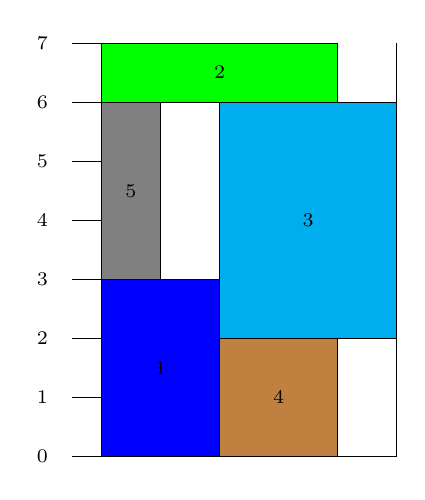
\begin{tikzpicture}[scale=0.75]
        \tikzstyle{every node} = [font=\scriptsize]
            \begin{scope}
                \foreach\x in {0,1,...,7}{
                    \draw (-0.5,\x) -- (0,\x);
                    \node at (-1,\x) {\x};
                }
               \draw (0 ,7) -- (0,0) -- (5,0) -- (5,7);
                   \filldraw[blue,draw=black] (0,0) rectangle (2,3);
                   \draw (1,1.5) node {1};

                   \filldraw[brown,draw=black] (2,0) rectangle (4,2);
                   \draw (3,1) node {4};

                   \filldraw[cyan,draw=black] (2,2) rectangle (5,6);
                   \draw (3.5,4) node {3};

                   \filldraw[gray,draw=black] (0,3) rectangle (1,6);
                   \draw (0.5,4.5) node {5};

                   \filldraw[green,draw=black] (0,6) rectangle (4,7);
                   \draw (2,6.5) node {2};

             \end{scope}
         \end{tikzpicture}
    \caption{Strip-packing solution example.}
    \label{fig:strip-packing}
\end{figure}
